% This example is meant to be compiled with lualatex or xelatex
% The theme itself also supports pdflatex
\PassOptionsToPackage{unicode}{hyperref}
\documentclass[aspectratio=1610, 12pt, xcolor=dvipsnames]{beamer}

% Warning, if another latex run is needed
% \usepackage[aux]{rerunfilecheck}

% just list chapters and sections in the toc, not subsections or smaller
\setcounter{tocdepth}{1}

%------------------------------------------------------------------------------
%------------------------------ Fonts, Unicode, Language ----------------------
%------------------------------------------------------------------------------
\usepackage{fontspec}
\defaultfontfeatures{Ligatures=TeX}  % -- becomes en-dash etc.

% german language
\usepackage{polyglossia}
\setdefaultlanguage{german}

% for english abstract and english titles in the toc
\setotherlanguages{english}

% intelligent quotation marks, language and nesting sensitive
\usepackage[autostyle]{csquotes}

% microtypographical features, makes the text look nicer on the small scale
\usepackage{microtype}

% colors and stuff
\usepackage{xcolor}
\usepackage[most]{tcolorbox}
% Here was colback=SpringGreen before but it is not finding the xcolor package
\tcbset{on line,
        boxsep=4pt, left=0pt,right=0pt,top=0pt,bottom=0pt,
        colframe=white,colback=green,
        highlight math style={enhanced}
        }
\newtcolorbox{mybox}[3][]
{
  colframe = #2!25,
  colback = #2!20,
  coltitle = #2!20!black,
  title = {#3},
  #1
}
%\colorlet{Green!40}
%------------------------------------------------------------------------------
%------------------------ Math Packages and settings --------------------------
%------------------------------------------------------------------------------

\usepackage{amsmath}
\usepackage{amssymb}
\usepackage{mathtools}
\usepackage{bbold}

% Enable Unicode-Math and follow the ISO-Standards for typesetting math
\usepackage[
  math-style=ISO,
  bold-style=ISO,
  sans-style=italic,
  nabla=upright,
  partial=upright,
]{unicode-math}
\setmathfont{Latin Modern Math}

% nice, small fracs for the text with \sfrac{}{}
\usepackage{xfrac}


%------------------------------------------------------------------------------
%---------------------------- Numbers and Units -------------------------------
%------------------------------------------------------------------------------

\usepackage[
  locale=DE,
  separate-uncertainty=true,
  per-mode=symbol-or-fraction,
]{siunitx}
\sisetup{math-micro=\text{µ},text-micro=µ}
% \sisetup{tophrase={{ to }}}
%------------------------------------------------------------------------------
%-------------------------------- tables  -------------------------------------
%------------------------------------------------------------------------------

\usepackage{booktabs}       % \toprule, \midrule, \bottomrule, etc

%------------------------------------------------------------------------------
%-------------------------------- graphics -------------------------------------
%------------------------------------------------------------------------------

\usepackage{graphicx}
%\usepackage{rotating}
\usepackage{grffile}
\usepackage{tikz}
\usepackage{circuitikz}
\usepackage{tikz-feynman}
\usepackage{subcaption}

% allow figures to be placed in the running text by default:
\usepackage{scrhack}
\usepackage{float}
\floatplacement{figure}{htbp}
\floatplacement{table}{htbp}

% keep figures and tables in the section
\usepackage[section, below]{placeins}

% smileys
\usepackage{MnSymbol,wasysym}

%------------------------------------------------------------------------------
%---------------------- customize list environments ---------------------------
%------------------------------------------------------------------------------

\usepackage{enumitem}
\usepackage{listings}
\usepackage{hepunits}

\usepackage{pdfpages}
%------------------------------------------------------------------------------
%------------------------------ Bibliographie ---------------------------------
%------------------------------------------------------------------------------

\usepackage[
  backend=biber,   % use modern biber backend
  autolang=hyphen, % load hyphenation rules for if language of bibentry is not
                   % german, has to be loaded with \setotherlanguages
                   % in the references.bib use langid={en} for english sources
]{biblatex}
\addbibresource{references.bib}  % the bib file to use
\DefineBibliographyStrings{german}{andothers = {{et\,al\adddot}}}  % replace u.a. with et al.


% Load packages you need here
% \usepackage{polyglossia}
% \setmainlanguage{german}

\usepackage{csquotes}


% \usepackage{amsmath}
% \usepackage{amssymb}
% \usepackage{mathtools}

\usepackage{hyperref}
\usepackage{bookmark}

% load the theme after all packages

\usetheme[
  showtotalframes, % show total number of frames in the footline
]{tudo}

% Put settings here, like
\unimathsetup{
  math-style=ISO,
  bold-style=ISO,
  nabla=upright,
  partial=upright,
  mathrm=sym,
}

% \setbeamertemplate{itemize item}{\scriptsize$\blacktriangleright$}
% \setbeamertemplate{itemize subitem}{\scriptsize$\blacktriangleright$}

%Titel:
\title{Bachelorseminar: Detektorsysteme und Hardwareprojekte}
%Autor
\author[N.Breer]{\textbf{Nils Breer}}
%Lehrstuhl/Fakultät
\institute{TU Dortmund}
%Titelgrafik muss ich einfueren!!!
%\titlegraphic{\includegraphics[width=0.3\textwidth]{content/Bilder/interferenz.jpg}}
\date{18.04.2023}

\begin{document}
\maketitle

\begin{frame}\frametitle{Vertex Locator (VELO)}
  \begin{itemize}
    \item $\bullet$\, Velo has 30 micro metre spatial hit resolution for 1 GeV transverse momentum
    \item $\bullet$\, primary vertex finding eff roughly 90%
    \item $\bullet$\, 52 modules with 4 hybrid pixel sensors each arranged in 2 havlves with 26 modules each
    \item $\bullet$\, can be opened by up to 30mm (3cm)
    \item $\bullet$\, VELO inside VELO tank and inside it's own pressure chamber, separated from the beam pipe vacuum with 150 micro metre thin aluminium foil
    \item $\bullet$\, can be close as near as 5.1 mm to the beam pipe for best possible vertex resolution
    \item $\bullet$\, open state for unstable beam conditions or if something is broken
  \end{itemize}
\end{frame}

\begin{frame}\frametitle{Scintillating Fibre Tracker (SciFi)}
  \begin{itemize}
    \item $\bullet$\, last element of the tracking system
    \item $\bullet$\, large tracking system consisting of 12 layers in 3 stations
    \item $\bullet$\, made out of scintillating fibre mats
    \item $\bullet$\, spatial mass resolution of 100 microns
    \item $\bullet$\, covering an area of 360 $m^2$
    \item $\bullet$\, $X1-U-V-X2$ layer pattern with $U-V$ stereo angles repeating for every station
  \end{itemize}
\end{frame}

\begin{frame}\frametitle{Upstream Tracker (UT)}
  \begin{itemize}
    \item $\bullet$\, silicon strip tracker with 100 - 200 micro metre pitch
    \item $\bullet$\, 4 tracking planes
    \item $\bullet$\, arranged in $X-U-V-X$ stereo pattern
    \item $\bullet$\, U and V are rotated by \pm 5 degrees too achieve 2D spatial resolution while suppressing ghost hits in reconstruction
    \item $\bullet$\, for momentum measurements there is a 4Tm (Tesla metre) integrated magnetic field between UT and SciFi
  \end{itemize}
\end{frame}

\begin{frame}\frametitle{Tracktypes}
  \begin{itemize}
    \item $\bullet$\, Tracks inside VELO: VELO track
    \item $\bullet$\, Long Tracks: extended VELO Tracks matches hits in UT and SciFi
    \item $\bullet$\, Upstream Tracks: Tracks that leave the Detector after passing the UT
    \item $\bullet$\, Tracks without hits in the VELO
    \begin{itemize}
      \item $\bullet$\, Downstream Tracks: Hits in UT and SciFi for long lived particles like Lambda and $K_s$
      \item $\bullet$\, TTracks: only Hits in SciFi, here the seeding algorithm is used
      \item $\bullet$\, TTracks found by seeding can also be found as long tracks by forward tracking
    \end{itemize}
    \item $\bullet$\, \to SciFi tracker has 99\% single hit efficiency
  \end{itemize}
\end{frame}

\begin{frame}\frametitle{Ring Immaging Cherenkov Detector}
  \begin{itemize}
    \item $\bullet$\, particle identification used to distinguish particles because track reco can only tell sign of particle change and momentum
    \item $\bullet$\, at interaction point: ring imiging cherenkov detector 1 and 2
    \item $\bullet$\, both detector volumes filled with flourcarbon gas \to HE particles generate cherenkov radiation
    \item $\bullet$\, emitted light is caught by Photomultipliers
    \item $\bullet$\, \to reconstruct speed \to reconstruct mass -> determine particle ID
    \item $\bullet$\, works good for: kaons, pions, protons
    \item $\bullet$\, RICH1 momentum range: 2 - 40 $GeV/c$ for high sensitivity
    \item $\bullet$\, RICH2 momentum range: 150 - 100 GeV/c and placed forther downstream as higher momentum particles are deflected less my magnet
  \end{itemize}
\end{frame}

\begin{frame}\frametitle{LumiTracker}
  \begin{itemize}
    \item $\bullet$\, lumitracker purpose: provide measurement of luminosity by operating independently from the rest of the LHCb experiment
    \item $\bullet$\, \to measures luminosity by reconstructing and counting tracks and also measures the luminous region by extending these tracks to the interaction point.
Reconstruction in real-time needed!
  \end{itemize}
\end{frame}

\begin{frame}\frametitle{TimePix4 Telescope}
  \begin{itemize}
    \item $\bullet$\, a
    \item $\bullet$\, b
    \item $\bullet$\, c
  \end{itemize}
\end{frame}

\begin{frame}\frametitle{Beam Conditions Monitor (BCM)}
  \begin{itemize}
    \item $\bullet$\, original: 2009 \to 2018
    \item $\bullet$\, not a detector taking physics data, but as safety measure
    \item $\bullet$\, situated in 2 stations upstream of magnet
    \item $\bullet$\, fast particle flux measurement system
    \item $\bullet$\, 2 rings with 8 diamond sensors at 2 z-positions around
    \item $\bullet$\, BCM-U is upstream of the VELO
    \item $\bullet$\, BCM-D is downsteam of of TT (previous \to now UT)
  \end{itemize}
\end{frame}

\begin{frame}\frametitle{BCM}
  \begin{itemize}
    \item $\bullet$\, 200 V bias voltage
    \item $\bullet$\, current through diamonds is read out by current-to-frequency converter (CFC) cards [these were originally designed for LHC beam loss monitor]
    \item $\bullet$\, CFC cards integration time = 40 micro seconds
    \item $\bullet$\, CFC cards measurement range = (2.5 pico Amp (pA), 1 milli Amp (mA))
    \item $\bullet$\, \to this is adequate for BCM diamonds since they show dark current in pico Amp range and dump threshold in micro Amp range
    \item $\bullet$\, digitized signal sent through redundant optical fibres with rate of 125kHz to TELL1 readout board
  \end{itemize}
\end{frame}

\begin{frame}\frametitle{BCM}
  \begin{itemize}
    \item $\bullet$\, firmware of TELL1 board applies "beam dump" logic to determine wether measured flux values are in problematic ranges
    \item $\bullet$\, TELL1 board located in D3 rack behind shielding wall in cavern where are UI is located
    \item $\bullet$\, Purpose of UI:
    \begin{itemize}
      \item $\bullet$\, when conditions are met TELL1 can request beam dump
      \item $\bullet$\, can inhibit injection of further bunches
      \item $\bullet$\, post-mortem trigger: request a snapshot of systems current data
      \item $\bullet$\, possible to send signal to VELO to open and move into safe position
    \end{itemize}
  \end{itemize}
\end{frame}

\begin{frame}\frametitle{BCM}
  \begin{itemize}
    \item $\bullet$\, during last months of LHC run 2 problems with BCM emerged
    \item $\bullet$\, multiple diamonds showed excessive currents during normal LHC conditions
    \item $\bullet$\, maybe radiation damage
  \end{itemize}
\end{frame}

\begin{frame}\frametitle{BCM upgrade}
  \begin{itemize}
    \item $\bullet$\, 2019 \to present
    \item $\bullet$\, all  subdetectors getting a new readout hardware
    \item $\bullet$\, TELL1 FPGA readout board is getting deprecated
    \item $\bullet$\, new LHCb wide used readout boards used -> PCIe40 (BCM40 is the variant for BCM called)
    \item $\bullet$\, this board will be implemented in the new data center above ground with CIBU stauing in the cavern it will need an extra component:
    \item $\bullet$\, MIBAD board: machine interface and beam abort decision board
    \item $\bullet$\, featuring Intel Arriva FPGA  will be placed in the same rack as TELL1 was previously
  \end{itemize}
\end{frame}

\begin{frame}\frametitle{BCM40 boards}
  \begin{itemize}
    \item $\bullet$\, handles low level parts of BCM system:
    \begin{itemize}
      \item $\bullet$\, receiving the read-out data
      \item $\bullet$\, implementing beam-dump logic
      \item $\bullet$\, interfacing to the machine
    \end{itemize}
    \item $\bullet$\, this data is tunneled to BCM40 at surface center
    \item $\bullet$\, Using BCM40 as interface to MIBAD board -> computer system housing BCM40 runs monitoring alowing observation and control of the whole system from
the LHCb control room
    \item $\bullet$\, \to sensitive components are placed so close to damaging beams that it needs to be continuously monitored \to BCM used for that
  \end{itemize}
\end{frame}

\begin{frame}\frametitle{MIBAD boards}
  \begin{itemize}
    \item $\bullet$\, d
    \item $\bullet$\, e
    \item $\bullet$\, f
  \end{itemize}
\end{frame}

\begin{frame}\frametitle{Diamond Fundamentals}
  \begin{itemize}
    \item $\bullet$\, bethe bloch for energy deposition
    \item $\bullet$\, crystalline carbon
    \item $\bullet$\, 2 displaced fcc lattices
    \item $\bullet$\, 43 eV needed to remove an atom from the lattice
    \item $\bullet$\, high mechanical hardness
    \item $\bullet$\, band gap of 5.47 eV indicates isulator but can be semiconductor as well
    \item $\bullet$\, large band gap \to low number of charge carriers \to low dark current
    \item $\bullet$\, large band gap + high displcement threshold \to very radiation hard
    \item $\bullet$\, CCE picture on page 30
  \end{itemize}
\end{frame}

\begin{frame}\frametitle{Diamonds and BCM}
  \begin{itemize}
    \item $\bullet$\, radiation damage \to sensors failed \to replacement of whole system
    \item $\bullet$\, to avoid said damage in the future:
    \item $\bullet$\, \to characterization of diamond sensors with charge collection efficiency
  \end{itemize}
\end{frame}

\begin{frame}\frametitle{Field Programmable Gate Arrays: FPGA}
  \begin{itemize}
    \item $\bullet$\, integrated digital circuits
    \item $\bullet$\, feature high number of reconfigurable logic blocks
    \item $\bullet$\, output depends on input (logic based)
    \item $\bullet$\, use look up table
    \item $\bullet$\, page 12 L Funke masterthesis: diagramm of FPGA
  \end{itemize}
\end{frame}

\begin{frame}\frametitle{}
  \begin{itemize}
    \item $\bullet$\,
    \item $\bullet$\,
    \item $\bullet$\,
  \end{itemize}
\end{frame}

\begin{frame}\frametitle{}
  \begin{itemize}
    \item $\bullet$\,
    \item $\bullet$\,
    \item $\bullet$\,
  \end{itemize}
\end{frame}

\begin{frame}\frametitle{}
  \begin{itemize}
    \item $\bullet$\,
    \item $\bullet$\,
    \item $\bullet$\,
  \end{itemize}
\end{frame}

\begin{frame}\frametitle{}
  \begin{itemize}
    \item $\bullet$\,
    \item $\bullet$\,
    \item $\bullet$\,
  \end{itemize}
\end{frame}

\begin{frame}\frametitle{}
  \begin{itemize}
    \item $\bullet$\,
    \item $\bullet$\,
    \item $\bullet$\,
  \end{itemize}
\end{frame}

\begin{frame}\frametitle{}
  \begin{itemize}
    \item $\bullet$\,
    \item $\bullet$\,
    \item $\bullet$\,
  \end{itemize}
\end{frame}

\begin{frame}\frametitle{}
  \begin{itemize}
    \item $\bullet$\,
    \item $\bullet$\,
    \item $\bullet$\,
  \end{itemize}
\end{frame}

\begin{frame}\frametitle{}
  \begin{itemize}
    \item $\bullet$\,
    \item $\bullet$\,
    \item $\bullet$\,
  \end{itemize}
\end{frame}

\begin{frame}\frametitle{}
  \begin{itemize}
    \item $\bullet$\,
    \item $\bullet$\,
    \item $\bullet$\,
  \end{itemize}
\end{frame}

\begin{frame}\frametitle{}
  \begin{itemize}
    \item $\bullet$\,
    \item $\bullet$\,
    \item $\bullet$\,
  \end{itemize}
\end{frame}

\begin{frame}\frametitle{}
  \begin{itemize}
    \item $\bullet$\,
    \item $\bullet$\,
    \item $\bullet$\,
  \end{itemize}
\end{frame}

\begin{frame}\frametitle{}
  \begin{itemize}
    \item $\bullet$\,
    \item $\bullet$\,
    \item $\bullet$\,
  \end{itemize}
\end{frame}

\begin{frame}\frametitle{}
  \begin{itemize}
    \item $\bullet$\,
    \item $\bullet$\,
    \item $\bullet$\,
  \end{itemize}
\end{frame}
% \begin{frame}\frametitle{Track hits comparison of V2 and simulation}
% \begin{mybox}{green}{}
%   \begin{itemize}
%     \item $\bullet$\, MC: hits on \textbf{reconstructed} tracks fill whole detector
%     \item $\bullet$\, data: filling tracks into A-side \to\, good!
%   \end{itemize}
% \end{mybox}
% \begin{mybox}{orange}{}
%   \begin{itemize}
%     \item \to\, scan C-side quarters for possible issues in distinct layers
%   \end{itemize}
% \end{mybox}
%   \begin{columns}
%     \begin{column}[c]{0.48\textwidth}
%       \begin{figure}
%         \centering
%         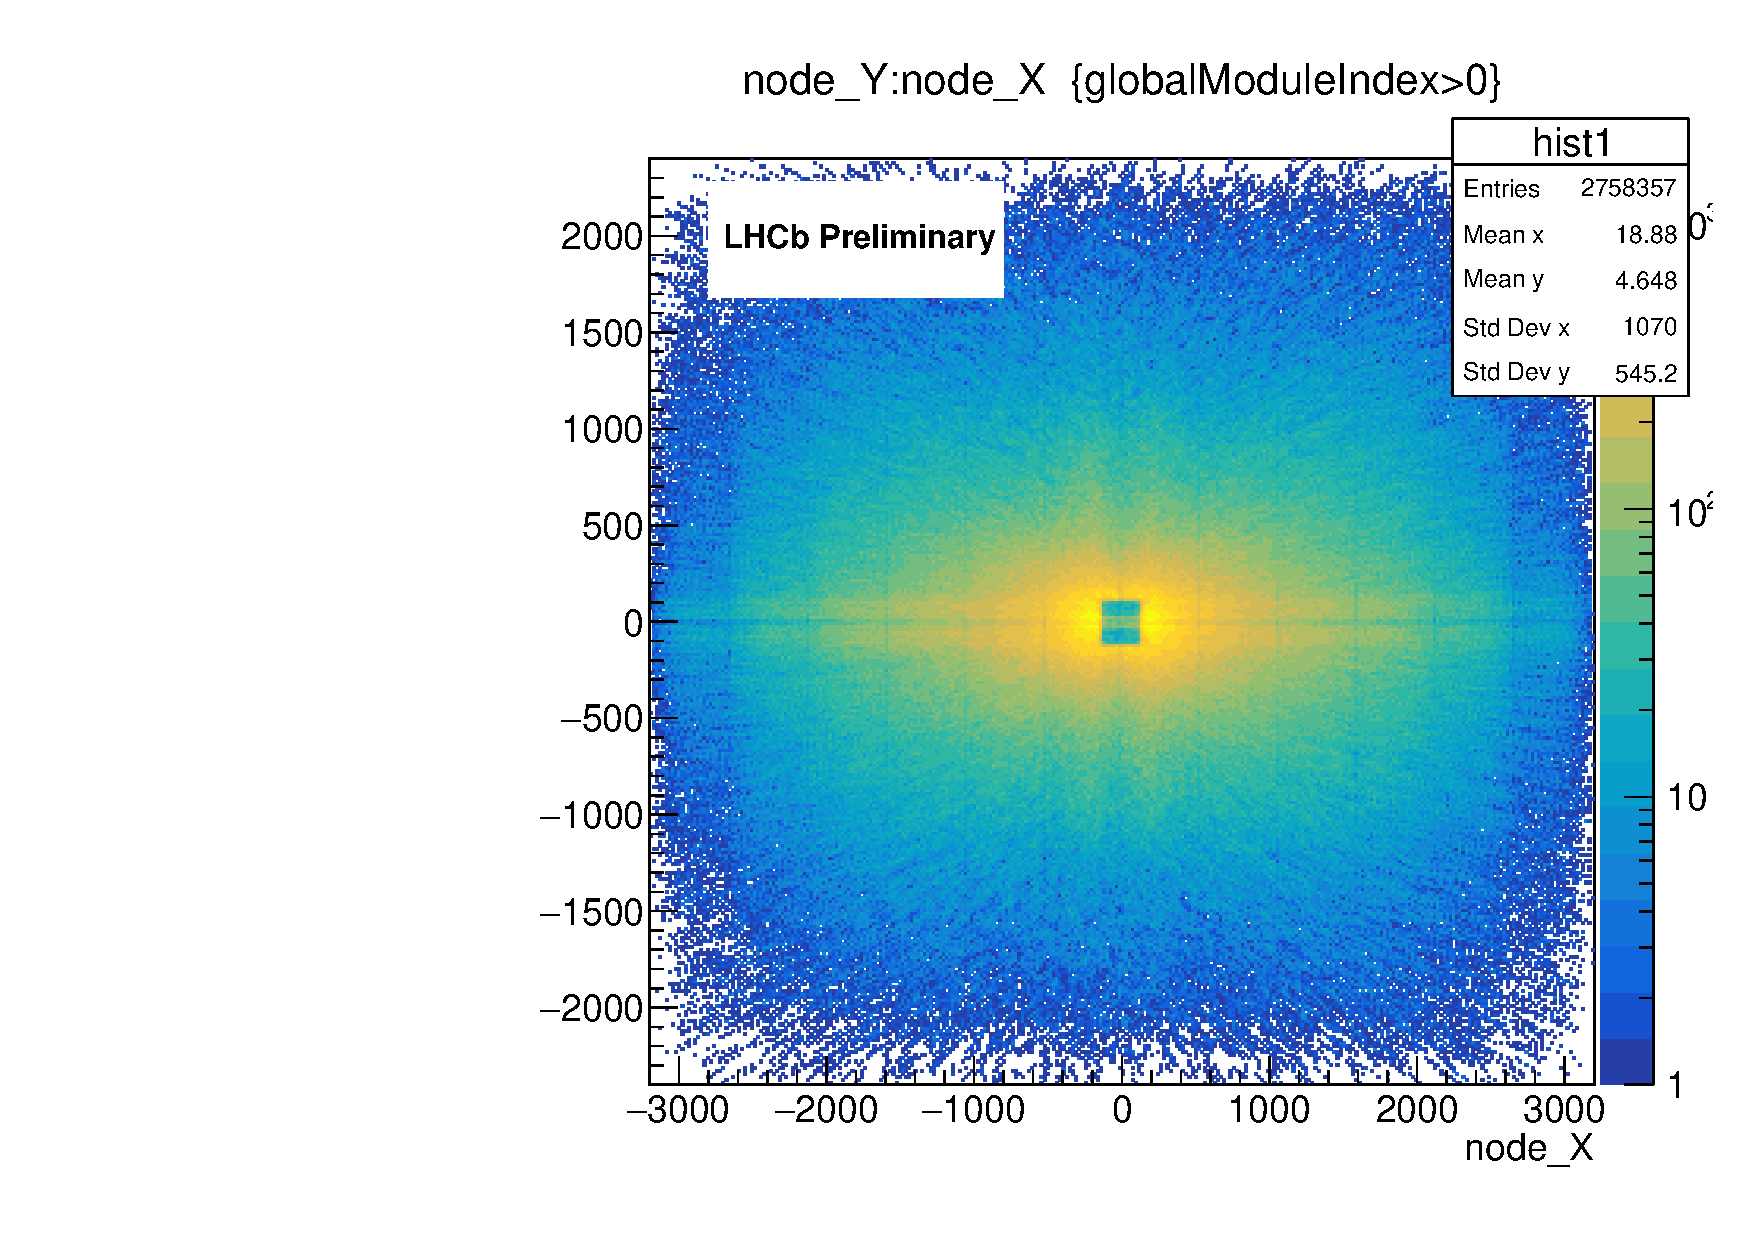
\includegraphics[width=0.6\textwidth]{logos/nodeXY_MC.pdf}%
%       \end{figure}
%     \end{column}
%     \begin{column}[c]{0.48\textwidth}
%       \begin{figure}
%         \centering
%         \includegraphics[width=0.6\textwidth]{tuples_out/combining_2D_nodeXY_v2.pdf}%
%       \end{figure}
%     \end{column}
%   \end{columns}
% \end{frame}

% \begin{frame}\frametitle{New Q0 positions in T2X2 layer}
%   \begin{itemize}
%     \item $\bullet$\, Changes based on V2 alignment positions
%     \item $\bullet$\, test incremental shifts of position/rotation until we found an improvement
%     \item $\bullet$\, rotations are with regard to the local frame of the module
%     \item $\bullet$\, positions: translations relative to the nominal position for each module
%     \item $\bullet$\, V2 alignment has only few tracks in Q0 because parts of the SciFi are too far out of alignment
%   \end{itemize}
%   \begin{figure}
%     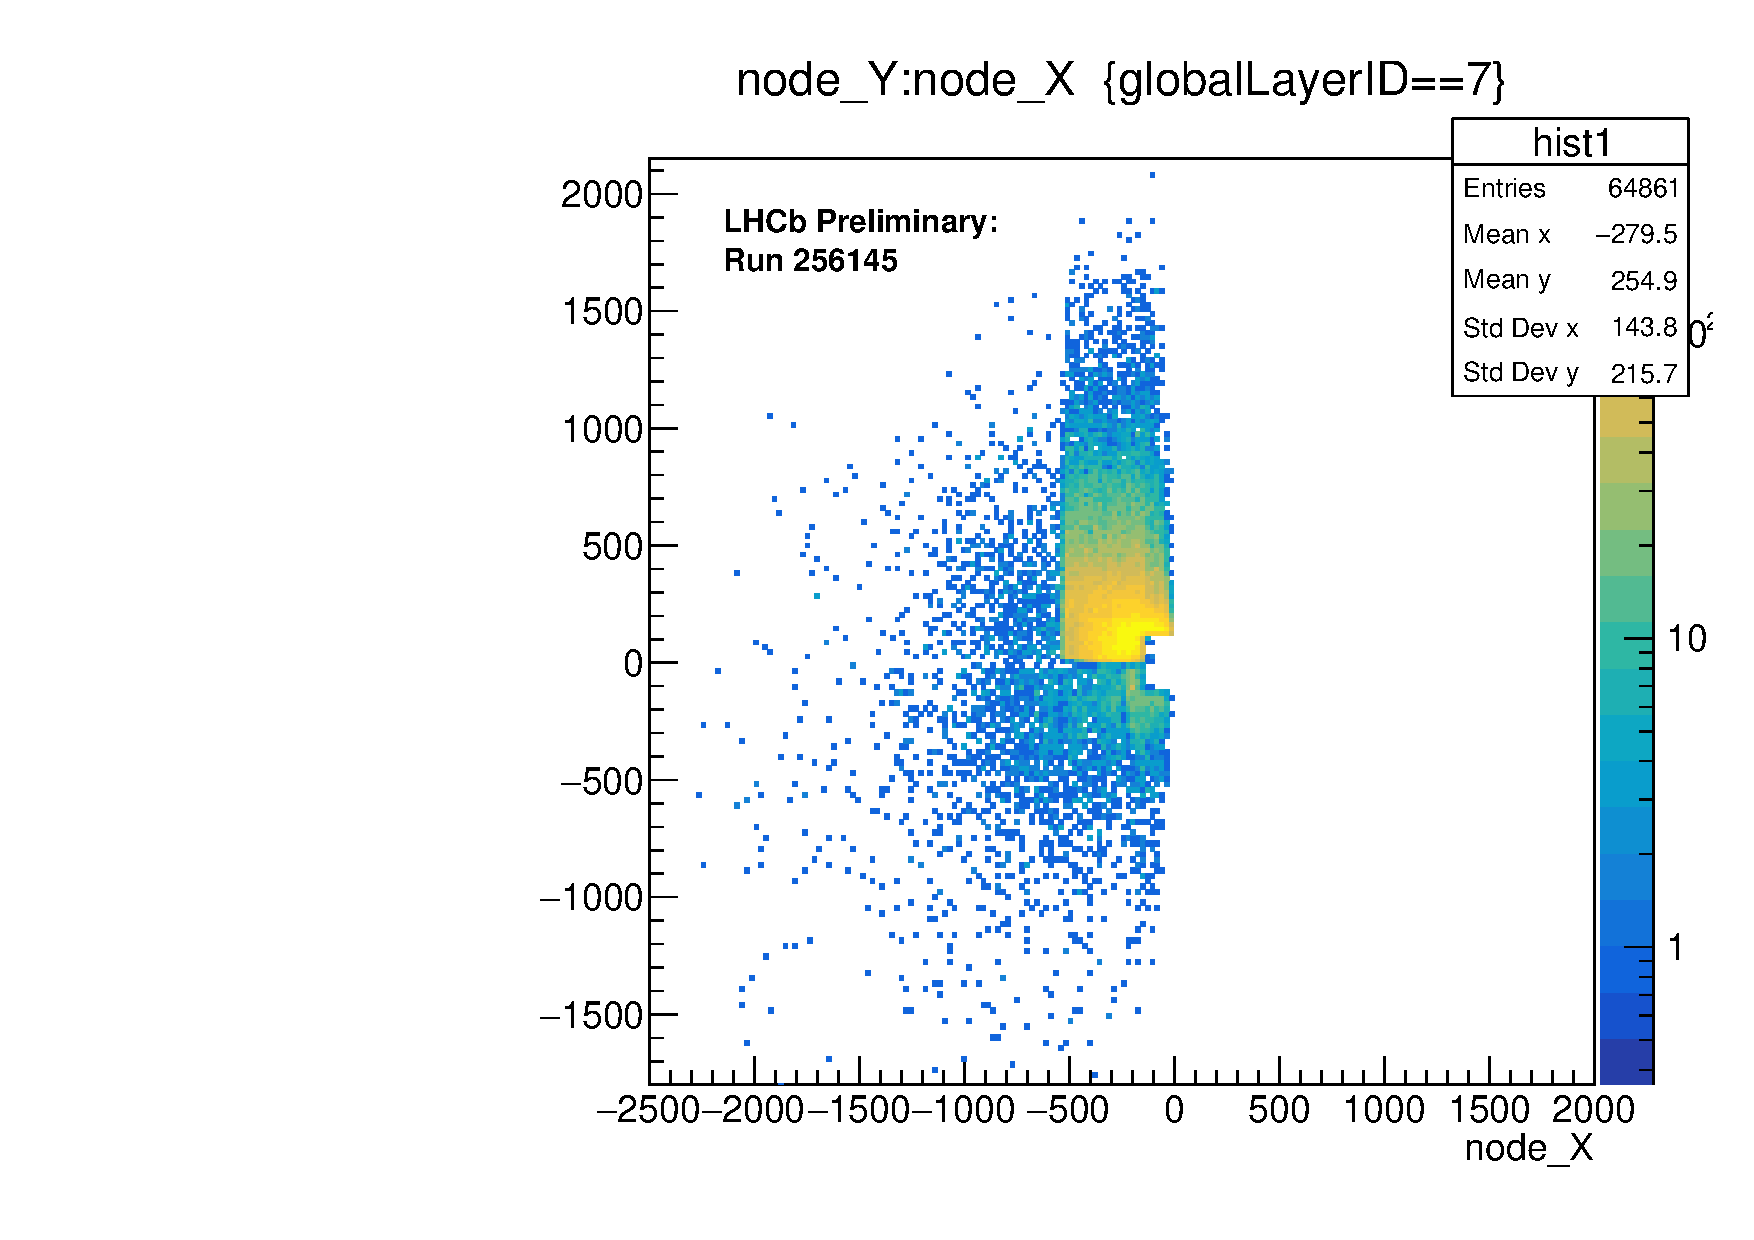
\includegraphics[width=0.26\textwidth]{logos/2D_nodeXY_v2_7_left.pdf}%
%     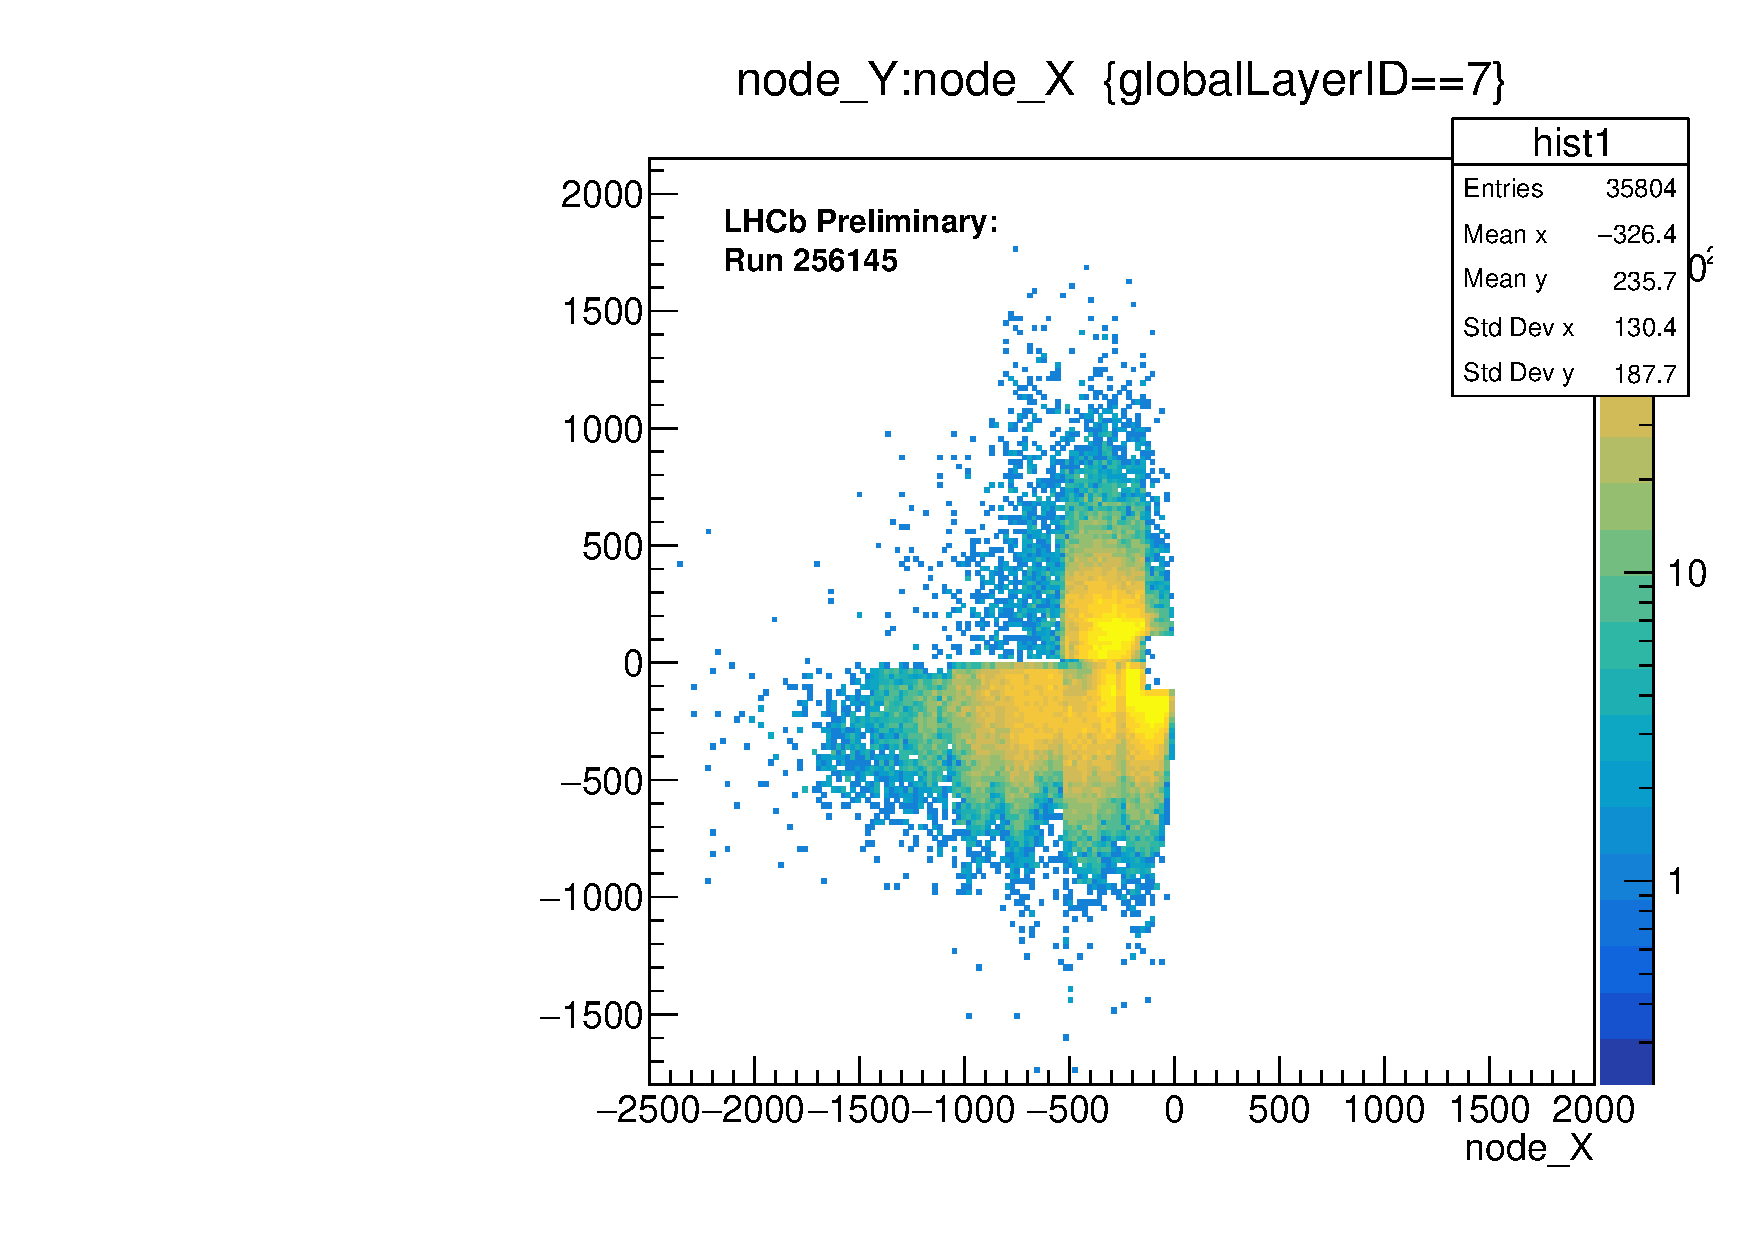
\includegraphics[width=0.26\textwidth]{logos/2D_nodeXY_quartermean_7_left.pdf}%
%     \includegraphics[width=0.26\textwidth]{problem_layer.png}%
%   \end{figure}
% \end{frame}

\end{document}
